%!TEX root = pset2.tex

\section{Logistic Regression}\label{sec:lr}

\subsection{Implementation}
We implemented $L_2$-regularized logistic regression using gradient descent.

\subsection{Testing in data with $\lambda = 0$}
We test the logistic regression 

\begin{figure}[h!]
\centering
    \begin{subfigure}[b]{0.4\textwidth}
	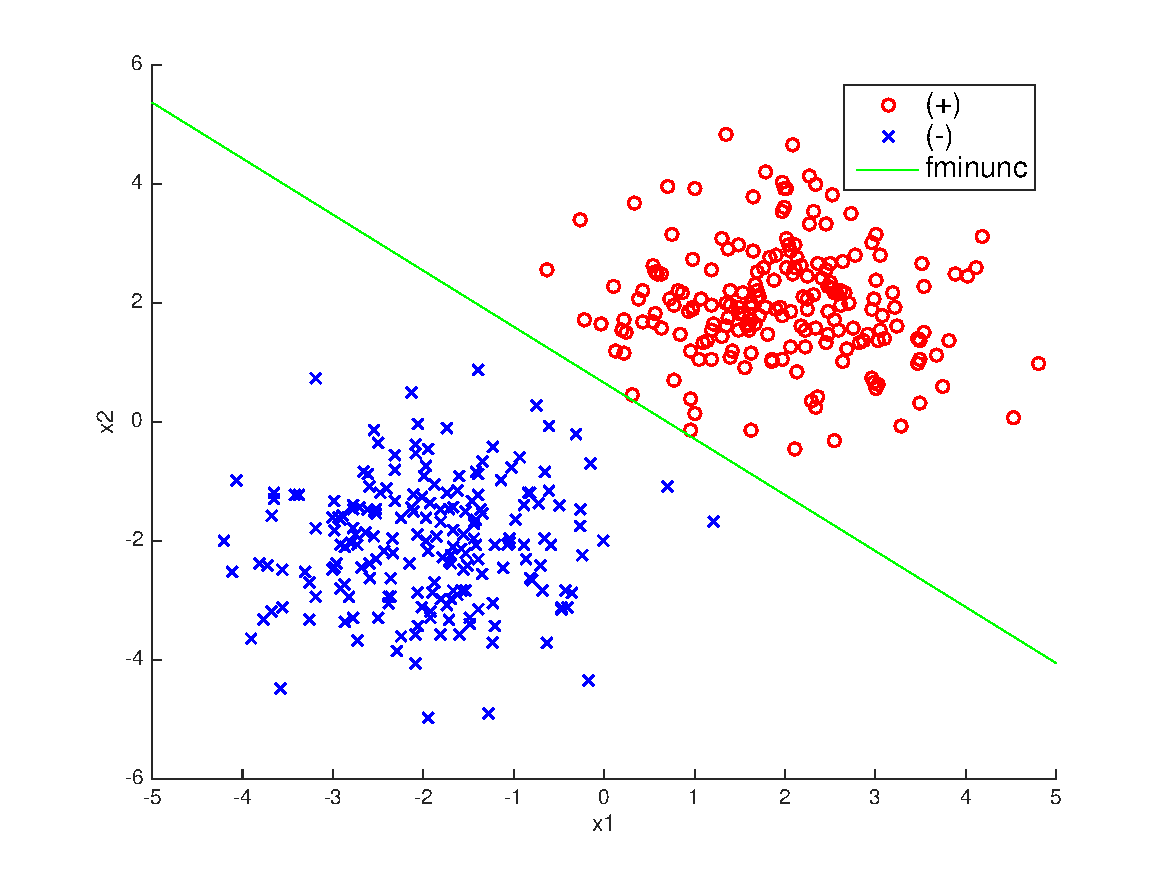
\includegraphics[scale=0.4]{hw2_11.pdf}
	\caption{Data with $\sigma = 1$}\label{fig:data_stdev1}
    \end{subfigure}
    \quad
    \begin{subfigure}[b]{0.4\textwidth}
	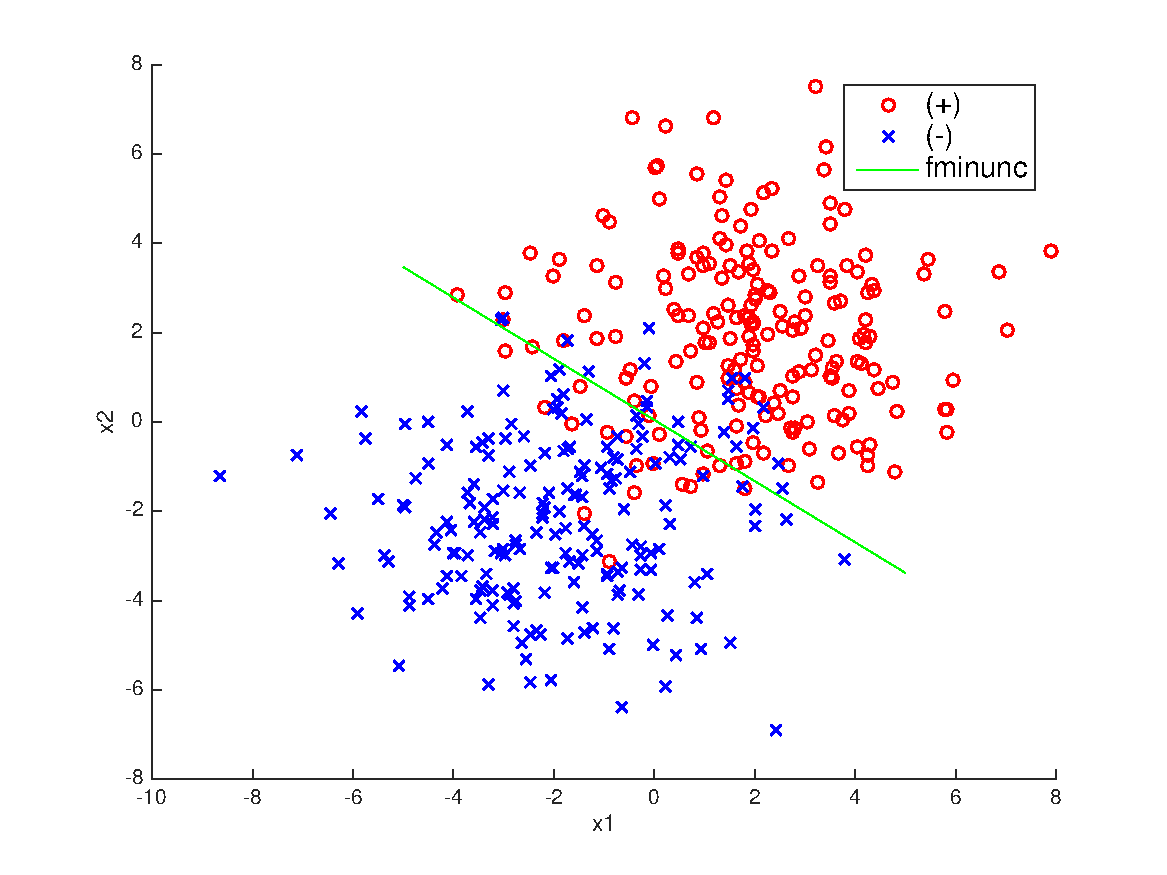
\includegraphics[scale=0.4]{hw2_12.pdf}
	\caption{CData with $\sigma = 2$}\label{fig:data_stdev2}
	\end{subfigure}
	
    \quad
    
    \begin{subfigure}[b]{0.4\textwidth}
	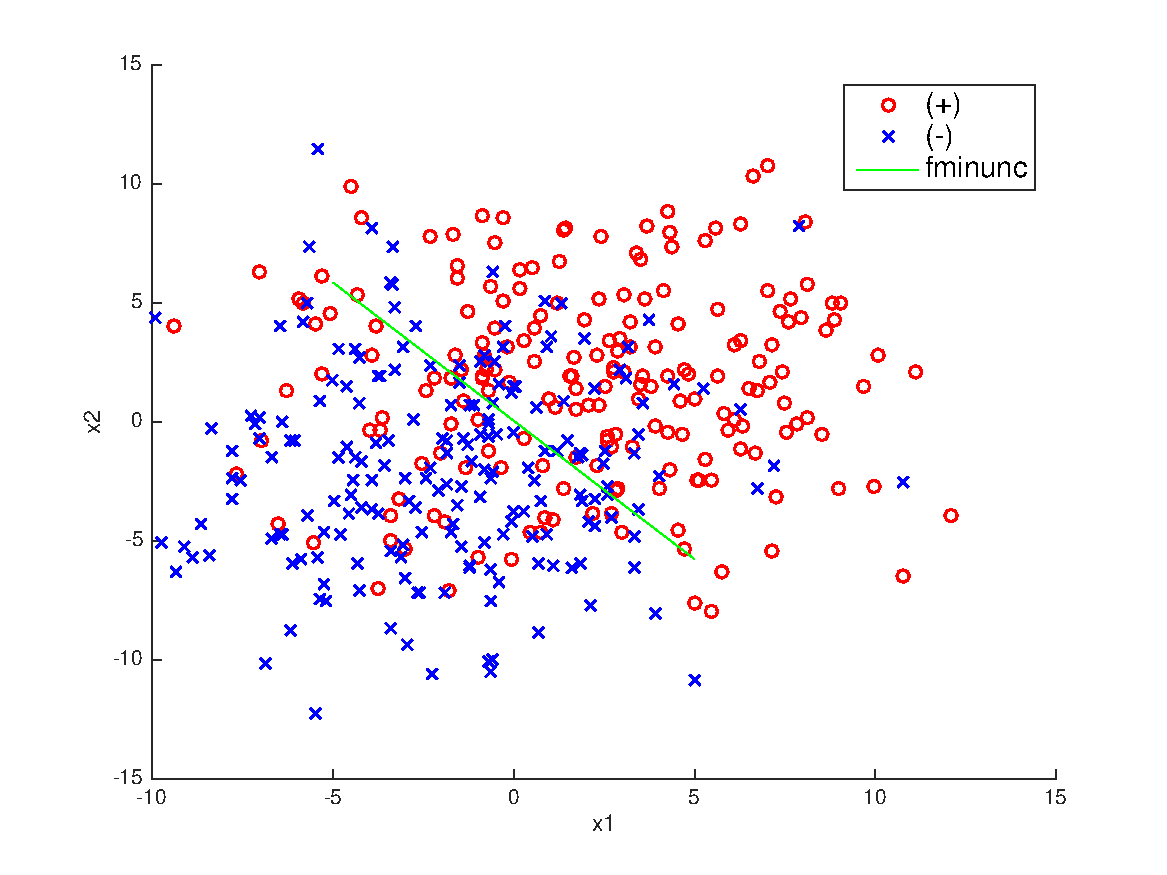
\includegraphics[scale=0.4]{hw2_13.pdf}
	\caption{Data with $\sigma = 4$}\label{fig:data_stdev4}
    \end{subfigure}  
    \quad
    \begin{subfigure}[b]{0.4\textwidth}
	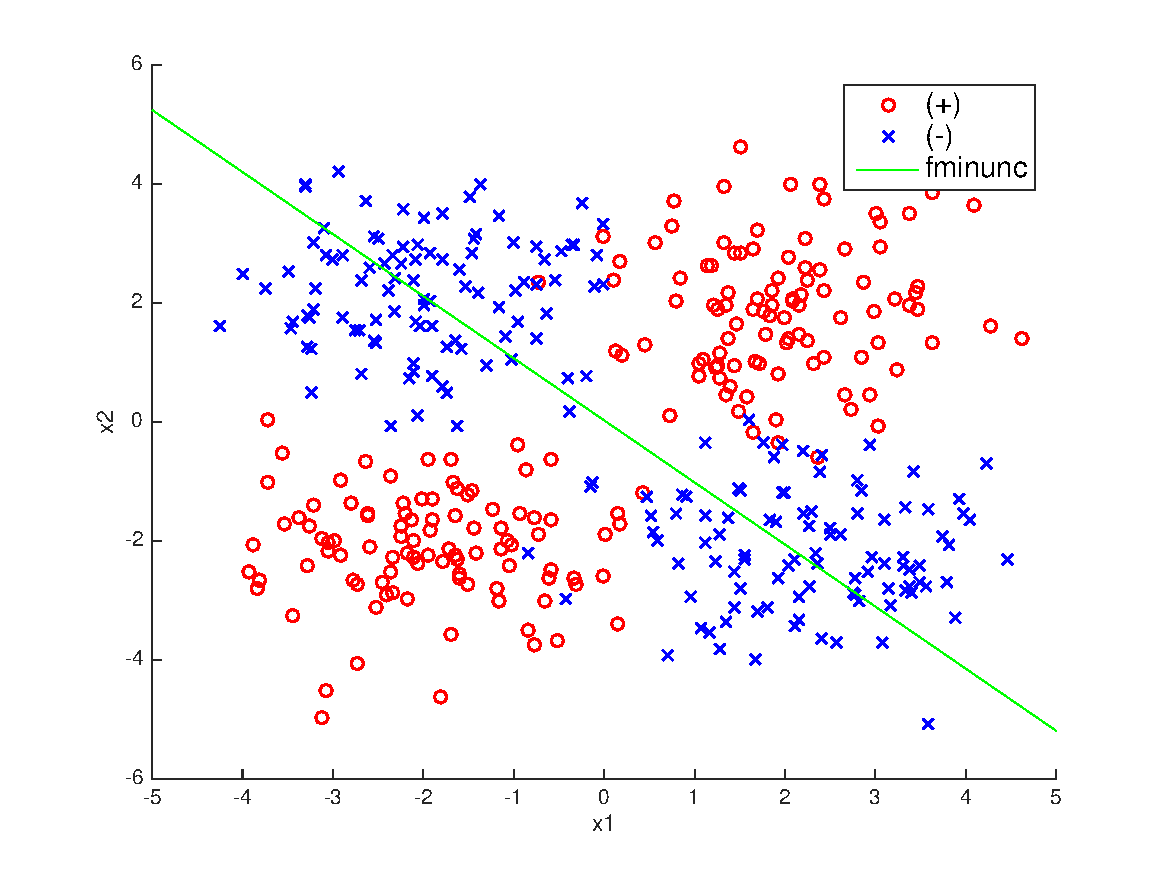
\includegraphics[scale=0.4]{hw2_14.pdf}
	\caption{Non-seperable data}\label{fig:data_nonsep}
    \end{subfigure}  
    \caption{}    
\end{figure}

